\section*{ÔN TẬP KIỂM TRA GIỮA KÌ 1 - ĐỀ 01}
\setcounter{ex}{0}\setcounter{bt}{0}
\noindent{\bf\fontfamily{qag}\selectfont\color{violet}A. PHẦN TRẮC NGHIỆM}
\Opensolutionfile{ans}[ans/ans-0-GK1-CanhDieu-De1-NH23-24]
\begin{ex}%[Dự Án 6 -Đề GHK1 - Khối 10]%[Huu Hien Maths]%[0C1Y1-2]%Câu 1
	Trong các câu sau, câu nào là mệnh đề?
	\choice
	{\True $10$ là số chính phương}
	{$a+b=c$}
	{$x^2-x=0$}
	{$2n+1$ chia hết cho $3$}
	\loigiai{
	Ta có $a+b=c$, $x^2-x=0$, $2n+1$ chia hết cho $3$ \textbf{không} phải là mệnh đề mà là mệnh đề chứa biến.
	}
\end{ex}
\begin{ex}%[Dự Án 6 -Đề GHK1 - Khối 10]%[Huu Hien Maths]%[0C1Y1-2]%Câu 2
	Các phương án sau, đâu là một mệnh đề đúng?
	\choice
	{$\dfrac{6}{3}=\dfrac{1}{2}$}
	{$2<1$}
	{\True $2+3=5$}
	{$3>5$}
	\loigiai{
		Mệnh đề đúng là $2+3=5$.
	}
\end{ex}
\begin{ex}%[Dự Án 6 -Đề GHK1 - Khối 10]%[Huu Hien Maths]%[0C1B1-2]%Câu 3
	Cho các mệnh đề sau đây:\\
	(I): Nếu tam giác $ABC$ đều thì $AB=AC$.\\
	(II): Nếu $a+b$ là các số chẵn thì $a,b$ là số chẵn.\\
	(III): Nếu tam giác $ABC$ có tổng hai góc bằng $90^{\circ}$ thì tam giác $ABC$ cân.\\
	Trong các mệnh đề trên, có bao nhiêu mệnh đề đúng?
	\choice
	{$0$}
	{$3$}
	{$2$}
	{\True $1$}
	\loigiai{
		Mệnh đề (I) là mệnh đề đúng.\\
		Mệnh đề (II) mệnh đề \textbf{sai} vì còn trường hợp $a,b$ là số lẻ.\\
		Mệnh đề (III) mệnh đề \textbf{sai} vì tam giác $ABC$ vuông chứ \textbf{không} phải là cân.\\
		Vậy chỉ có $1$ mệnh đề đúng.
	}
\end{ex}
\begin{ex}%[Dự Án 6 -Đề GHK1 - Khối 10]%[Huu Hien Maths]%[0C1Y1-3]%Câu 4
	Mệnh đề phủ định của mệnh đề: ``$\forall x \in \mathbb{N},x^2 \geq x$'' là
	\choice
	{$\forall x \in \mathbb{N},x^2 \leq x$}
	{$\exists x \in \mathbb{N},x^2 \geq x$}
	{$\exists x \in \mathbb{N},x^2 \leq x$}
	{\True $\exists x \in \mathbb{N},x^2<x$}
	\loigiai{
		Mệnh đề: ``$\forall x \in \mathbb{N},x^2 \geq x$'' có mệnh đề phủ định là ``$\exists x \in \mathbb{N},x^2<x$''.
	}
\end{ex}
\begin{ex}%[Dự Án 6 -Đề GHK1 - Khối 10]%[Huu Hien Maths]%[0C1Y1-2]%Câu 5
	Trong các mệnh đề sau, mệnh đề nào \textbf{sai}?
	\choice
	{Nếu cả hai số chia hết cho $3$ thì tổng hai số đó chia hết cho $3$}
	{Nếu hai tam giác bằng nhau thì chúng có diện tích bằng nhau}
	{Nếu một số có tận cùng bằng $0$ thì nó chia hết cho $5$}
	{\True Nếu một số chia hết cho $5$ thì nó có tận cùng bằng $0$}
	\loigiai{
		Nếu một số chia hết cho $5$ thì nó có tận cùng bằng $0$ là đáp án  \textbf{sai}, vì một số chia hết cho $5$ có thể có tận cùng là $5$.
	}
\end{ex}
\begin{ex}%[Dự Án 6 -Đề GHK1 - Khối 10]%[Huu Hien Maths]%[0C1Y1-2]%Câu 6
	Cho mệnh đề $P \colon$ ``$\forall x \in \mathbb{R} \colon x^2+x+1 \ne 0$''. Mệnh đề phủ định của mệnh đề $P$ và tính đúng, sai của nó là
	\choice
	{\True $\overline{P} \colon$ ``$\exists x \in \mathbb{R} \colon x^2+x+1=0$'' và $\overline{P}$ là mệnh đề \textbf{sai}}
	{$\overline{P} \colon$ ``$\exists x \in \mathbb{R} \colon x^2+x+1=0$'' và $\overline{P}$ là mệnh đề đúng}
	{$\overline{P} \colon$ ``$\exists x \in \mathbb{R} \colon x^2+x+1 \ne 0$'' và $\overline{P}$ là mệnh đề đúng}
	{$\overline{P} \colon$ ``$\forall x \in \mathbb{R} \colon x^2+x+1=0$'' và $\overline{P}$ là mệnh đề \textbf{sai}}
	\loigiai{
		Phủ định của mệnh đề $P \colon$ ``$\forall x \in \mathbb{R} \colon x^2+x+1 \ne 0$'' là $\overline{P} \colon$ ``$\exists x \in \mathbb{R} \colon x^2+x+1=0$''.\\
		có $x^2+x+1=\left( x+\dfrac{1}{2} \right)^2+\dfrac{3}{4}>0,\,\forall x \in \mathbb{R}$ nên mệnh đề $\overline{P} \colon $ ``$\exists x \in \mathbb{R} \colon x^2+x+1=0$'' sai vì phương trình $x^2+x+1=0$ vô nghiệm nên không tồn tại $x \in \mathbb{R}$ để phương trình $x^2+x+1=0$.
	}
\end{ex}
\begin{ex}%[Dự Án 6 -Đề GHK1 - Khối 10]%[Huu Hien Maths]%[0C1Y2-1]%Câu 7
	Viết tập hợp $B=\left\{ x \in \mathbb{Q}/(x^2-2)(2x^2-5x+3)=0 \right\}$ bằng cách liệt kê các phần tử của tập hợp.
	\choice
	{\True $B=\left\{ 1;\dfrac{3}{2} \right\}$}
	{$B=\left\{ \dfrac{3}{2} \right\}$}
	{$B=\big\{1\big\}$}
	{$B=\left\{ 1;\dfrac{3}{2};\sqrt{2};-\sqrt{2} \right\}$}
	\loigiai{
		Xét $(x^2-2)(2x^2-5x+3)=0$ $\Leftrightarrow \hoac{&x^2-2=0\\&2x^2-5x+3=0} \Leftrightarrow \hoac{&x=\pm \sqrt{2} \notin \mathbb{Q}\\&x=1 \in \mathbb{Q}\\&x=\dfrac{3}{2} \in \mathbb{Q}}$.Vậy $B=\left\{ 1;\dfrac{3}{2} \right\}$.
	}
\end{ex}
\begin{ex}%[Dự Án 6 -Đề GHK1 - Khối 10]%[Huu Hien Maths]%[0C1Y2-1]%Câu 8
	Cho tập hợp $A=\left\{ 2x+3|x \in \mathbb{N},x \leq 5 \right\}$. Tập hợp A là
	\choice
	{$A=\big\{1;2;3;4;5\big\}$}
	{$A=\big\{1;3;5;7;9;11\big\}$}
	{$A=\big\{3;4;5;6;7;8\big\}$}
	{\True $A=\big\{3;5;7;9;11;13\big\}$}
	\loigiai{
		Xét $x \in \mathbb{N}$ và $x \leq 5$ nên $x \in \big\{0;1;2;3;4;5\big\}$. Do đó $A=\big\{3;5;7;9;11;13\big\}$.
	}
\end{ex}
\begin{ex}%[Dự Án 6 -Đề GHK1 - Khối 10]%[Huu Hien Maths]%[0C1Y2-1]%Câu 9
	Hãy liệt kê các phần tử của tập hợp $X=\left\{ x \in \mathbb{Z}|7x^2-5x-2=0 \right\}$.
	\choice
	{$X=\big\{0\big\}$}
	{\True $X=\big\{1\big\}$}
	{$X=\left\{ 1;\dfrac{1}{2} \right\}$}
	{$X=\left\{ 1;-\dfrac{2}{7} \right\}$}
	\loigiai{
		Xét phương trình: $7x^2-5x-2=0 \Leftrightarrow \hoac{&x=1\\&x=-\dfrac{2}{7}.}$\\
		Do $x \in \mathbb{Z}$ nên $X=\big\{1\big\}$.
	}
\end{ex}
\begin{ex}%[Dự Án 6 -Đề GHK1 - Khối 10]%[Huu Hien Maths]%[0C1Y2-3]%Câu 10
	Cho hai tập hợp $A=\left\{ n \in \mathbb{N}\bigg|n \leq 50,n \vdots 6 \right\}$ và $B=\big\{6;12;18;24;30;36;42;48\big\}$. Mệnh đề nào sau đây đúng?
	\choice
	{\True $B \subset A$}
	{$A \subset B$}
	{$A=B$}
	{$A\bigcap B=\varnothing$}
	\loigiai{
		Ta có $A=\big\{0;6;12;18;24;30;36;42;48\big\}$ $\Rightarrow B \subset A$.
	}
\end{ex}
\begin{ex}%[Dự Án 6 -Đề GHK1 - Khối 10]%[Huu Hien Maths]%[0C1Y2-2]%Câu 11
	Tập hợp nào sau đây có đúng hai tập hợp con?
	\choice
	{$\left\{ x;\varnothing \right\}$}
	{\True $\big\{x\big\}$}
	{$\left\{ x;y;\varnothing \right\}$}
	{$\big\{x;y\big\}$}
	\loigiai{
		$\big\{x\big\}$ có hai tập con là $\big\{x\big\}$ và $\varnothing$.
	}
\end{ex}
\begin{ex}%[Dự Án 6 -Đề GHK1 - Khối 10]%[Huu Hien Maths]%[0C1Y2-3]%Câu 12
	Cho $A=\big\{-1;1;5\big\};B=\big\{0;1;3;5\big\}$. Khẳng định nào sau đây đúng?
	\choice
	{$A \cap B=\big\{1\big\}$}
	{$A \cap B=\big\{1;3\big\}$}
	{\True $A \cap B=\big\{1;5\big\}$}
	{$A \cap B=\big\{1;3;5\big\}$}
	\loigiai{
		$A=\big\{1;5\big\};B=\big\{1;3;5\big\}$. Suy ra $A \cap B=\big\{1;5\big\}$.
	}
\end{ex}
\begin{ex}%[Dự Án 6 -Đề GHK1 - Khối 10]%[Huu Hien Maths]%[0C1Y2-3]%Câu 13
	Cho hai tập hợp $A=\big\{0;2\big\},B=\big\{0;1;2;3;4\big\}$. Số tập hợp $X$ thỏa mãn $A \cup X=B$ là
	\choice
	{$2$}
	{$3$}
	{\True $4$}
	{$5$}
	\loigiai{
		\immini{Vì $A \cup X=B$ nên $X$ bắt buộc phải chứa các phần tử $\big\{1;3;4\big\}$ và $X \subset B$.\\
		Vậy X có $4$ tập hợp đó là $\big\{0;1;2;3;4\big\},\big\{1;2;3;4\big\},\big\{1;3;4\big\},\big\{0;1;3;4\big\}$.}
		{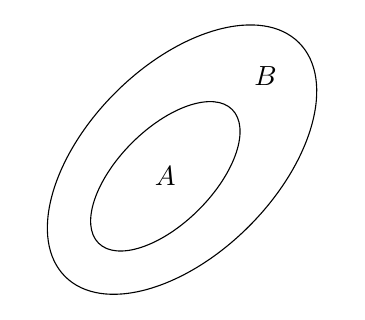
\begin{tikzpicture}[scale=0.6, line join=round, line cap=round]
				\draw[rotate=45] (0,0) ellipse (2cm and 1cm) (0,0) node{$A$}; 
				\draw[rotate=45] (0.5,0) ellipse (3.5cm and 2cm) (3,0) node{$B$}; 
		\end{tikzpicture}	}
	}
\end{ex}
\begin{ex}%[Dự Án 6 -Đề GHK1 - Khối 10]%[Huu Hien Maths]%[0C1Y2-4]%Câu 14
	Cho $A=\big\{1;3;5;7\big\}$; $B=\big\{1;2;3;4;5;6\big\}$. Tập hợp $B \setminus A$ có số phần tử là
	\choice
	{$1$}
	{$4$}
	{$2$}
	{\True $3$}
	\loigiai{
		Ta có $B \setminus A=\big\{2;4;6\big\}$\\
		Suy ra tập hợp $B \setminus A$ có 3 phần tử.
	}
\end{ex}
\begin{ex}%[Dự Án 6 -Đề GHK1 - Khối 10]%[Huu Hien Maths]%[0C1Y2-4]%Câu 15
	Cho hai tập hợp $A=\big\{1;2;4;6\big\},B=\big\{1;2;3;4;5;6;7;8\big\}$ khi đó tập $C_BA$ là
	\choice
	{\True $\big\{3;5;7;8\big\}$}
	{$\big\{4;6\big\}$}
	{$\big\{2;6;7;8\big\}$}
	{$\big\{1;2;4;6\big\}$}
	\loigiai{
		Ta có $C_BA=\big\{3;5;7;8\big\}$.
	}
\end{ex}
\begin{ex}%[Dự Án 6 -Đề GHK1 - Khối 10]%[Huu Hien Maths]%[0C1B2-5]%Câu 16
	Một lớp học có $25$ học sinh giỏi môn Toán, $23$ học sinh giỏi môn Lý, $14$ học sinh giỏi cả môn Toán và Lý và có $6$ học sinh không giỏi môn nào cả. Hỏi lớp đó có bao nhiêu học sinh?
	\choice
	{$54$}
	{\True $40$}
	{$26$}
	{$68$}
	\loigiai{
		\immini{Gọi T, L lần lượt là tập hợp các học sinh giỏi Toán và các học sinh giỏi Lý.\\
		Ta có\\
		$|T|$: là số học sinh giỏi Toán\\
		$|L|$: là số học sinh giỏi Lý\\
		$\left| T \cap L \right|$: là số học sinh giỏi cả hai môn Toán và Lý\\
		Khi đó số học sinh của lớp là $\left| T \cup L \right|+6$.}
		{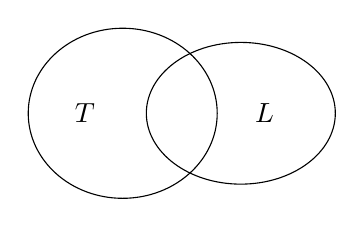
\begin{tikzpicture}[scale=0.6, line join=round, line cap=round]
				\draw[rotate=0] (0,0) ellipse (2cm and 1.8cm) (-0.8,0) node{$T$}; 
				\draw[rotate=0] (2.5,0) ellipse (2cm and 1.5cm) (3,0) node{$L$}; 
		\end{tikzpicture}	}
		Mà $\left| T \cup L \right|=|T|+|L|-\left| T \cap L \right|=25+23-14=34$.\\
		Vậy số học sinh của lớp là $34+6=40$.
	}
\end{ex}
\begin{ex}%[Dự Án 6 -Đề GHK1 - Khối 10]%[Huu Hien Maths]%[0C1Y2-6]%Câu 17
	Cho tập hợp $A=(-\infty;3]; B=(1;5]$. Khi đó, tập $A \cup B$ là
	\choice
	{$(1;3]$}
	{$(3;5]$}
	{\True $(-\infty;5]$}
	{$(-\infty;1)$}
	\loigiai{
		Ta có $A \cup B=(-\infty;5]$.\\
		.
	}
\end{ex}
\begin{ex}%[Dự Án 6 -Đề GHK1 - Khối 10]%[Huu Hien Maths]%[0C1Y2-6]%Câu 18
	Cho tập hợp $A=(-2;6);B= [-3;4]$. Khi đó, tập $A \cap B$ là
	\choice
	{$(-2;3]$}
	{\True $(-2;4]$}
	{$(-3;6]$}
	{$(4;6]$}
	\loigiai{
		Ta có $A \cap B=(-2;4]$.
	}
\end{ex}
\begin{ex}%[Dự Án 6 -Đề GHK1 - Khối 10]%[Huu Hien Maths]%[0C1Y2-6]%Câu 19
	Cho tập $A=(4;7]$ và $B=(-3;5]$. Tập $A \setminus B$ là
	\choice
	{$(-3;4]$}
	{$(4;5]$}
	{$(-3;7]$}
	{\True $(5;7]$}
	\loigiai{
		Ta có $A \setminus B=$ $(4;7] \setminus (-3;5]=(5;7]$.
	}
\end{ex}
\begin{ex}%[Dự Án 6 -Đề GHK1 - Khối 10]%[Huu Hien Maths]%[0C1Y2-7]%Câu 20
	Cho tập $A=(-5;8]$ và $B=(-2;4]$. Tập $C_AB$ là
	\choice
	{$C_AB=(-5;-2) \cup (4;8)$}
	{$C_AB=(-5;-2) \cup (4;8]$}
	{$C_AB=(-5;-2] \cup (4;8)$}
	{\True $C_AB=(-5;-2] \cup (4;8]$}
	\loigiai{
	Ta có	$C_AB=A \setminus B=(-5;8] \setminus (-2;4]=(-5;-2] \cup (4;8]$.
	}
\end{ex}
\begin{ex}%[Dự Án 6 -Đề GHK1 - Khối 10]%[Huu Hien Maths]%[0C2Y1-2]%Câu 21
	Cặp số nào sau đây \textbf{không} phải là nghiệm của bất phương trình $2x+3y-1<0$
	\choice
	{$x=0;y=0$}
	{$x=1;y=-1$}
	{$x=0;y=-2$}
	{\True $x=-1;y=1$}
	\loigiai{
		Thử các cặp số $(x;y)$ vào bất phương trình $2x+3y-1<0$.\\
		Ta có  $2\cdot(-1)+3\cdot1-1=0$ nên $x=-1;y=1$ \textbf{không} phải là nghiệm của bất phương trình $2x+3y-1<0$.
	}
\end{ex}
\begin{ex}%[Dự Án 6 -Đề GHK1 - Khối 10]%[Huu Hien Maths]%[0C2Y2-1]%Câu 22
	\immini
	{
	Cho hình vẽ bên dưới, miền nghiệm được biểu diễn bởi phần không bị tô màu (không có đường thẳng) là miền nghiệm của bất phương trình nào sau đây?	
	\choice
	{\True $x+y>2$}
	{$x+y \geq 2$}
	{$x+y \leq 2$}
	{$x+y<2$}
	}
	{
	\begin{tikzpicture}[scale=.65, font=\footnotesize, line join=round, line cap=round, >=stealth]
		\def\a{-1}\def\b{2}
		%\draw[color=gray,dash pattern=on 1pt off 1pt,xstep=1.0cm,ystep=1.0cm] (-5.2,-5.2) grid (5.2,5.2);
		\draw[->] (-2,0) -- (5,0) node[below] {$x$};
		\draw[->] (0,-2) -- (0,4) node[left] {$y$};
		\draw[thick,samples=150,smooth,domain=-2:4] plot(\x,{\a*\x+(\b)});
		\draw[pattern = north west lines,draw=none] (-2,4)--(-2,-2)--(4,-2)--cycle;
		\fill (0,0) circle (1pt) node[below left]{$O$};
		\fill (2,0) circle (1pt) node[above]{$2$};
		\fill (0,2) circle (1pt) node[above right]{$2$};
	\end{tikzpicture}
	}
	\loigiai{
		Ta thấy đường thẳng đi qua hai điểm $A(0;2)$ và $B(2;0)$ nên đường thẳng có phương trình $\Delta \colon x+y-2=0$.\\
		Lấy điểm $O(0;0) \notin \Delta$, không thuộc miền nghiệm của bất phương trình và ta có $0+0<2$ nên hình trên biểu diễn miền nghiệm của bất phương trình $x+y>2$.
	}
\end{ex}
\begin{ex}%[Dự Án 6 -Đề GHK1 - Khối 10]%[Huu Hien Maths]%[0C2B1-2]%Câu 23
	\immini
	{
	Miền không bị gạch (không tính đường thẳng) được cho bởi hình sau, là miền nghiệm của bất phương trình nào?
	\choice
	{$2x+y-6>0$}
	{\True $2x+y-6<0$}
	{$x+2y-6<0$}
	{$x+2y-6>0$}
	}
	{
	\begin{tikzpicture}[scale=.65,yscale=0.65, font=\footnotesize, line join=round, line cap=round, >=stealth]
		\def\a{-2}\def\b{6}
		%\draw[color=gray,dash pattern=on 1pt off 1pt,xstep=1.0cm,ystep=1.0cm] (-5.2,-5.2) grid (5.2,5.2);
		\draw[->] (-1,0) -- (3.5,0) node[below] {$x$};
		\draw[->] (0,-1) -- (0,8) node[left] {$y$};
		\draw[thick,samples=150,smooth,domain=-1:3.5] plot(\x,{\a*\x+(\b)});
		\draw[pattern = north west lines,draw=none] (-1,8)--(3.5,-1)--++(90:9)--cycle;
		\fill (0,0) circle (1pt) node[below left]{$O$};
		\fill (3,0) circle (1pt) node[below]{$3$};
		\fill (0,6) circle (1pt) node[left]{$6$};
	\end{tikzpicture}
	}
	\loigiai{
		Từ đồ thị ta thấy:\\
		Đường thẳng $d$ đi qua $2$ điểm $A(3;0)$, $B(0;6)$ suy ra phương trình là $2x+y-6=0$.\\
		Điểm $O(0;0)$ thuộc miền nghiệm của bất phương trình.\\
		Nên đáp án là $2x+y-6<0$.
	}
\end{ex}
\begin{ex}%[Dự Án 6 -Đề GHK1 - Khối 10]%[Huu Hien Maths]%[0C2Y2-1]%Câu 24
	Miền nghiệm của hệ bất phương trình $\heva{&3x-2y+6 \geq 0\\&2x+y-10 \geq 0\\&y-1>0}$ là miền chứa điểm nào trong các điểm sau?
	\choice
	{$M(1;-3)$}
	{\True $N(4;3)$}
	{$P(-1;5)$}
	{$Q(-2;-3)$}
	\loigiai{
		Thay $x=1$, $y=-3$ vào từng hệ bất phương trình đã cho, ta được:\\
		$\heva{&15 \geq 0\\&-11 \geq 0\\&-4>0}$ (không thoả mãn).\\
		Thay $x=4$, $y=3$ vào từng hệ bất phương trình đã cho, ta được:\\
		$\heva{&12 \geq 0\\&1 \geq 0\\&2>0}$ (thoả mãn).\\
		Thay $x=-1$, $y=5$ vào từng hệ bất phương trình đã cho, ta được:\\
		$\heva{&-7 \geq 0\\&-7 \geq 0\\&4>0}$ (không thoả mãn).\\
		PThay $x=-2$, $y=-3$ vào từng hệ bất phương trình đã cho, ta được:\\
		$\heva{&6 \geq 0\\&-17 \geq 0\\&-4>0}$ (không thoả mãn).\\
		Vậy miền nghiệm của hệ bất phương trình $\heva{&3x-2y+6 \geq 0\\&2x+y-10 \geq 0\\&y-1>0}$ là miền chứa điểm $N(4;3)$.
	}
\end{ex}
\begin{ex}%[Dự Án 6 -Đề GHK1 - Khối 10]%[Huu Hien Maths]%[0C2K2-2]%Câu 25
	Trong một cuộc thi pha chế, mỗi đội chơi được sử dụng tối đa $24$g hương liệu, $9$ lít nước và $210$g đường để pha chế nước cam và nước táo. Để pha chế $1$ lít nước cam cần $30$g đường, $1$ lít nước và $1$g hương liệu; Để pha chế $1$ lít nước táo cần $10$g đường, $1$ lít nước và $4$g hương liệu. Mỗi lít nước cam nhận được $60$ điểm thưởng, mỗi lít nước táo nhận được $80$ điểm thưởng. Hỏi cần pha chế bao nhiêu lít nước trái cây mỗi loại để đạt được số điểm thưởng cao nhất?
	\choice
	{$5$ lít nước cam và $4$ lít nước táo}
	{$6$ lít nước cam và $5$ lít nước táo}
	{\True $4$ lít nước cam và $5$ lít nước táo}
	{$4$ lít nước cam và $6$ lít nước táo}
	\loigiai{
		Giả sử $x,y$ là số lít nước cam và số lít nước táo mà mỗi đội cần pha chế.\\
		Suy ra $30x+10y$ là số gam đường cần dùng;\\
		$x+y$ là số lít nước cần dùng;\\
		$x+4y$ là số gam hương liệu cần dùng.\\
		Theo giả thiết ta có $\heva{&x \geq 0\\&y \geq 0\\&30x+10y \leq 210\\&x+y \leq 9\\&x+4y \leq 24} \Leftrightarrow \heva{&x \geq 0\\&y \geq 0\\&3x+y \leq 21\\&x+y \leq 9\\&x+4y \leq 24} \cdot (*)$\\
		Số điểm thưởng nhận được sẽ là $P=60x+80y$.\\
		Trong mặt phẳng tọa độ $Oxy$, vẽ các đường thẳng:\\
		$(d) \colon 3x+y-21=0,(d') \colon x+y-9=0,(\vartriangle) \colon x+4y-24=0$\\
		Khi đó miền nghiệm của hệ bất phương trình (*) là phần mặt phẳng (ngũ giác $OABCD$) tô màu trên hình vẽ
		\begin{center}
			\begin{tikzpicture}[scale=.651,yscale=1, font=\footnotesize, line join=round, line cap=round, >=stealth]
				%\def\a{-2}\def\b{6}
				%\draw[color=gray,dash pattern=on 1pt off 1pt,xstep=1.0cm,ystep=1.0cm] (-5.2,-5.2) grid (5.2,5.2);
				\clip (-2,-2) rectangle (9.5,9.5);
				\draw[->] (-2,0) -- (9.25,0) node[above] {$x$};
				\draw[->] (0,-2) -- (0,9.25) node[right] {$y$};
				\draw[thick,samples=150,smooth,domain=-2:9.5] plot(\x,{9-\x});
				\draw[thick,samples=150,smooth,domain=-2:9.5] plot(\x,{21-3*\x});
				\draw[thick,samples=150,smooth,domain=-2:9.5] plot(\x,{6-0.25*\x});
				\draw[pattern = north west lines,pattern color=gray,draw=none] (0,0)--(7,0)--(6,3)--(4,5)--(0,6)--cycle;
				\fill (0,0) circle (1pt) node[below left]{$O$};
				\fill (0,6) circle (1pt) node[above right]{$A$};
				\fill (4,5) circle (1pt) node[above]{$B$};
				\fill (6,3) circle (1pt) node[right]{$C$};
				\fill (7,0) circle (1pt) node[above right]{$D$};
				\fill (7,0) circle (1pt) node[below]{$7$};
				\fill (4,0) circle (1pt) node[below]{$4$};
				\fill (6,0) circle (1pt) node[below]{$6$};
				\fill (0,6) circle (1pt) node[above left]{$6$};
				\fill (0,5) circle (1pt) node[left]{$5$};
				\fill (0,3) circle (1pt) node[left]{$3$};
				\draw[dashed] (4,0)--(4,5)--(0,5);
				\draw[dashed] (6,0)--(6,3)--(0,3);
			\end{tikzpicture}
		\end{center}
		Xét các đỉnh của miền khép kín tạo ra bởi hệ (*) là 		$O(0;0),A(0;6),B(4;5),C(6;3),D(7;0)$\\
		Ta thấy $P$ đạt giá trị lớn nhất tại $x=4,y=5$. \\
		Vậy để đạt được số điểm thưởng cao nhất cần pha chế $4$ lít nước cam và $5$ lít nước táo.
	}
\end{ex}
\begin{ex}%[Dự Án 6 -Đề GHK1 - Khối 10]%[Huu Hien Maths]%[0C4Y1-2]%Câu 26
	Cho $\sin x=\dfrac{2}{5}$ và $90^{\circ}<x<180^{\circ}$. Tính giá trị cosx.
	\choice
	{$\dfrac{\sqrt{21}}{5}$}
	{$\sqrt{21}$}
	{\True $-\dfrac{\sqrt{21}}{5}$}
	{$\dfrac{1}{5}$}
	\loigiai{
		$\sin^2x+\cos^2x=1 \Leftrightarrow \cos^2x=1-\sin^2x \Leftrightarrow \cos^2x=1-\dfrac{4}{25} \Leftrightarrow \cos^2x=\dfrac{21}{25} \Leftrightarrow \cos x=\pm \dfrac{\sqrt{21}}{5}$.\\
		Vì $90^{\circ}<x<180^{\circ}$ nên $\cos x<0$. Vậy $\cos x=-\dfrac{\sqrt{21}}{5}$.
	}
\end{ex}
\begin{ex}%[Dự Án 6 -Đề GHK1 - Khối 10]%[Huu Hien Maths]%[0C4B2-1]%Câu 27
	Cho $\triangle ABC$ có $b=6,c=8,\widehat{A}=60^{\circ}$. Tính độ dài cạnh $a$.
	\choice
	{\True $2\sqrt{13}$}
	{$3\sqrt{12}$}
	{$2\sqrt{37}$}
	{$\sqrt{20}$}
	\loigiai{
	Ta có $a^2=b^2+c^2-2bc\cos A=36+64-2 \cdot 6 \cdot 8 \cdot \cos 60^{\circ}=52 \Rightarrow a=2\sqrt{13}$.
	}
\end{ex}
\begin{ex}%[Dự Án 6 -Đề GHK1 - Khối 10]%[Huu Hien Maths]%[0C4B2-1]%Câu 28
	Cho tam giác $ABC$ thoả mãn: $b^2+c^2-a^2=\sqrt{3}bc$. Khi đó:
	\choice
	{\True $A=30^{\circ}$}
	{$A=45^{\circ}$}
	{$A=60^{\circ}$}
	{$A=75^{\circ}$}
	\loigiai{
		Ta có 	$\cos A=\dfrac{b^2+c^2-a^2}{2bc}=\dfrac{\sqrt{3}bc}{2bc}=\dfrac{\sqrt{3}}{2} \Rightarrow \widehat{A}=30^{\circ}$.
	}
\end{ex}
\begin{ex}%[Dự Án 6 -Đề GHK1 - Khối 10]%[Huu Hien Maths]%[0C1Y2-7]%Câu 29
	Cho hai tập hợp $A=(1;5];B=(2;7]$. Tập hợp $A \setminus B$ là
	\choice
	{\True $(1;2]$}
	{$(2;5)$}
	{$(-1;7]$}
	{$(-1;2)$}
	\loigiai{
		Ta có 	$A \setminus B=\left\{ x \in \mathbb{R} \setminus x \in A \text{ và } x \notin B \right\} \Rightarrow x \in (1;2]$. .
	}
\end{ex}
\begin{ex}%[Dự Án 6 -Đề GHK1 - Khối 10]%[Huu Hien Maths]%[0C4B2-1]%Câu 30
	Cho $\triangle ABC$ có $AB=5$; $\widehat{A}=40^{\circ}$; $\widehat{B}=60^{\circ}$. Độ dài $BC$ gần nhất với kết quả nào?
	\choice
	{$3,7$}
	{\True $3,3$}
	{$3,5$}
	{$3,1$}
	\loigiai{
		Ta có $\widehat{C}=180^{\circ}-\widehat{A}-\widehat{B}=180^{\circ}-40^{\circ}-60^{\circ}=80^{\circ}$\\
		Áp dụng định lý sin: $\dfrac{BC}{\sin A}=\dfrac{AB}{\sin C} \Rightarrow BC=\dfrac{AB}{\sin C} \cdot \sin A=\dfrac{5}{\sin 80^{\circ}}\sin 40^{\circ} \approx 3{,}3$.
	}
\end{ex}
\begin{ex}%[Dự Án 6 -Đề GHK1 - Khối 10]%[Huu Hien Maths]%[0C4B2-1]%Câu 31
	Cho tam giác $ABC$, biết độ dài của cạnh $BC$ là $a=10$ và bán kính đường tròn ngoại tiếp tam giác là $R=10$. Tính số đo góc $\widehat{A}$.
	\choice
	{\True $\widehat{A}=30^{\circ}$}
	{$\widehat{A}=45^{\circ}$}
	{$\widehat{A}=60^{\circ}$}
	{$\widehat{A}=90^{\circ}$}
	\loigiai{
		Áp dụng định lý sin ta có $\sin \widehat{A}=\dfrac{a}{2R}=\dfrac{10}{20}=\dfrac{1}{2}$ $\Rightarrow \widehat{A}=30^{\circ}$.
	}
\end{ex}
\begin{ex}%[Dự Án 6 -Đề GHK1 - Khối 10]%[Huu Hien Maths]%[0C4B2-1]%Câu 32
	Cho tam giác $ABC$, biết độ dài của ba cạnh của tam giác là $a=10$, $b=8$, $c=9$. Số đo góc $\widehat{A}$ gần nhất với kết quả nào sau đây.
	\choice
	{\True $72^{\circ}$}
	{$68^{\circ}$}
	{$86^{\circ}$}
	{$34^{\circ}$}
	\loigiai{
		Áp dụng định lý cô-sin ta có $\cos A=\dfrac{8^2+9^2-10^2}{2 \cdot 8 \cdot 9}=\dfrac{5}{16}$ $\Rightarrow \widehat{A} \approx 72^{\circ}$.
	}
\end{ex}
\begin{ex}%[Dự Án 6 -Đề GHK1 - Khối 10]%[Huu Hien Maths]%[0C4B2-1]%Câu 33
	Cho tam giác $ABC$, biết bán kính đường tròn ngoại tiếp tam giác là $R=10$, diện tích tam giác $ABC$ bằng 50 và $\widehat{A}=30^{\circ}$. Tính khoảng cách từ đỉnh $A$ đến cạnh $BC$.
	\choice
	{$15$}
	{$20$}
	{\True $10$}
	{$\dfrac{19}{2}$}
	\loigiai{
		Gọi d là khoảng cách từ đỉnh $A$ đến cạnh $BC$.\\
		Áp dụng định lý sin ta có $a=2R\sin A=2 \cdot 10 \cdot \sin 30^{\circ}=10$.\\
		Mặt khác $S_{\triangle ABC}=\dfrac{1}{2} \cdot a \cdot d$.\\
		Suy ra $d=\dfrac{2S_{\triangle ABC}}{a}=\dfrac{2 \cdot 50}{10}=10$\\
		Vậy khoảng cách từ đỉnh $A$ đến cạnh $BC$ là $d=10$.
	}
\end{ex}
\begin{ex}%[Dự Án 6 -Đề GHK1 - Khối 10]%[Huu Hien Maths]%[0C4B2-1]%Câu 34
	Cho tam giác $ABC$ có $BC=a;CA=b;AB=c$. Khẳng định nào sau đây là đúng?
	\choice
	{$S=bc\sin A$}
	{$b=\dfrac{2R}{\sin B}$}
	{$S=\sqrt{p(p+a)(p+b)(p+c)}$}
	{\True $a^2=b^2+c^2-2bc\cos A$}
	\loigiai{
		Áp dụng định lí cô-sin ta có công thứuc $a^2=b^2+c^2-2bc\cos A$ là đúng.
	}
\end{ex}
\begin{ex}%[Dự Án 6 -Đề GHK1 - Khối 10]%[Huu Hien Maths]%[0C4B2-1]%Câu 35
	\immini{Cho tam giác $ABC$ có $AC=3;BC=4;S_{ABC}=3\sqrt{3}$. Tính độ dài cạnh $AB$.}
	{\begin{tikzpicture}[scale =2]
			\clip (-2,-1) rectangle (2,.8);
			\draw (-1.6,-.5)coordinate [label=left:\tiny $A$] (A)--(.2,.48)coordinate [label=left:\tiny $B$] (B)--(1.1,-.5)coordinate [label=right:\tiny $C$] (C)--cycle;
			\node at (-.8,0) [above]{\tiny ?};
			\node at (.85,0) [above]{\tiny $3$};
			\node at (-.2,-.8) [above]{\tiny $4$};
	\end{tikzpicture}}
	\choice
	{$13$}
	{$\sqrt{37}$}
	{\True $\sqrt{13}$}
	{$37$}
	\loigiai{
		Ta có $S_{ABC}=\dfrac{1}{2}AC \cdot BC \cdot \sin C$ $=\dfrac{1}{2} \cdot 3 \cdot 4\sin C$ $=3\sqrt{3}$ $\Rightarrow \sin C=\dfrac{\sqrt{3}}{2}$ $\Rightarrow \widehat{C}=60^{\circ}$.\\
		Áp dụng định lý cô-sin trong tam giác $ABC$, ta có
		\begin{eqnarray*}
		AB^2&=&BC^2+AC^2-2 \cdot BC \cdot AC \cdot \cos C \\
			&=&3^2+4^2-2 \cdot 3 \cdot 4 \cdot \cos 60^{\circ}\\
			&=&3^2+4^2-2 \cdot 3 \cdot 4 \cdot \dfrac{1}{2}=13.
		\end{eqnarray*}
		Do đó $AB=\sqrt{13}$.	
	}
\end{ex}
\Closesolutionfile{ans}
\noindent{\bf\fontfamily{qag}\selectfont\color{violet}B. PHẦN TỰ LUẬN}
\begin{bt}
	Tìm tập xác định các hàm số sau:
	\begin{enumEX}{2}
		\item $y=\dfrac{x-2}{\sqrt{x^2+2x+1}}$.
		\item $y=\dfrac{\sqrt{1-2x}}{x^2-4x+3}$
	\end{enumEX}
	\loigiai{
		
	}
\end{bt}
\begin{bt}%[Dự Án 6 -Đề GHK1 - Khối 10]%[Huu Hien Maths]%[0C2K2-2]%Câu 2
	Một công ty dự kiến chi $500$ triệu đồng cho một đợt quảng cáo sản phẩm của mình. Biết rằng chi phí cho một block $1$ phút quảng cáo trên đài phát thanh là $10$ triệu đồng và chi phí cho một block $10$ giây quảng cáo trên đài truyền hình là $25$ triệu đồng. Đài phát thanh chỉ nhận các chương trình quảng cáo với ít nhất $5$ block, đài truyền hình chỉ nhận các chương trình quảng cáo với số block ít nhất là $10$. Lệp hệ bất phương trình biểu diễn mỗi liên hệ trên và biểu diễn miền nghiệm của chúng?
	\loigiai{
		Gọi $x,y$ tương ứng là số block công ty đó thuê quảng cáo trên đài đài phát thanh và đài truyền hình. Chi phí công ty cần bỏ ra là $10x+25y$ (triệu đồng).\\
		Mức chi phí cho quảng cáo không quá $500$ triệu nên $10x+25y \leq 500$ hay $2x+5y \leq 100$.\\
		Do các điều kiện đài phát thanh và đài truyền hình đưa ra nên $x \geq 5;y \geq 10;x,y \in \mathbb{N}$.\\
		Ta được hệ bất phương trình
		$\heva{&2x+5y \leq 100\\&x \geq 5\\&y \geq 10}(*)$.\\
		Biểu diễn miền nghiệm của hệ (*) như hình sau
		\begin{center}
			\begin{tikzpicture}[scale=0.65,xscale=.2,yscale=.2, font=\footnotesize, line join=round, line cap=round, >=stealth]
				%\def\a{-2}\def\b{6}
				%\draw[color=gray,dash pattern=on 1pt off 1pt,xstep=1.0cm,ystep=1.0cm] (-5.2,-5.2) grid (5.2,5.2);
				\clip (-10,-10) rectangle (60,31);
				\draw[->] (-5,0) -- (58,0) node[above] {$x$};
				\draw[->] (0,-5) -- (0,30) node[right] {$y$};
				%\draw[thick,samples=150,smooth,domain=-2:9.5] plot(\x,{9-\x});
				\draw[thick,samples=150,smooth,domain=-5:56] plot(\x,{20-0.4*\x});
				%\draw[thick,samples=150,smooth,domain=-2:9.5] plot(\x,{6-0.25*\x});
				\draw[pattern = north west lines,pattern color=gray,draw=none] (5,18)--(25,10)--(5,10)--cycle;		
				\fill (0,0) circle (1pt) node[below left]{$O$};
				\draw (-5,10)--(56,10) (5,-5) -- (5,30);
				\draw[dashed] (25,0)--(25,10)--(0,10) (0,18)--++(0:5);
				\fill (5,18) circle (1.5pt) node[above right]{$A$};
				\fill (25,10) circle (1.5pt) node[above]{$B$};
				\fill (5,10) circle (1.5pt) node[below right]{$C$};
				\fill (0,10) circle (1.5pt) node[above left]{$10$};
				\fill (0,20) circle (1.5pt) node[above left]{$20$};
				\fill (0,18) circle (1.5pt) node[left]{$18$};
				\fill (5,0) circle (1.5pt) node[below right]{$5$};
				\fill (25,0) circle (1.5pt) node[below]{$25$};
				\fill (50,0) circle (1.5pt) node[below]{$50$};
			\end{tikzpicture}
		\end{center}
		Miền nghiệm của hệ (*) là miền tam giác ABC với $A(5;18)$; $B(25;10)$ và $C(5;10)$.\\
	}
\end{bt}
\begin{bt}%[Dự Án 6 -Đề GHK1 - Khối 10]%[Huu Hien Maths]%[0C4K2-1]%Câu 3
	Cho tam giác $ABC$ có $AC=8$ và có góc $\widehat{A}=120^{\circ}$. Trên đoạn $AB$ lấy điểm $M$ sao cho $AM=\dfrac{2}{3}AB$. Biết diện tích tam giác $\triangle BMC$ bằng $S_{\triangle BMC}=4\sqrt{3}$. Chứng minh rằng $S_{\triangle BMC}=\dfrac{1}{3}S_{\triangle ABC}$. Tính độ dài cạnh $AB$.
	\loigiai{
		\immini{
		Ta có $AM=\dfrac{2}{3}AB \Rightarrow BM=\dfrac{1}{3}AB$ từ đó $S_{\triangle BMC}=\dfrac{1}{3}S_{\triangle ABC}=4\sqrt{3} \Rightarrow S_{\triangle ABC}=12\sqrt{3}$.\\
		Áp dụng công thức diện tích ta có
		\begin{eqnarray*}
			S_{\triangle ABC}&=&\dfrac{1}{2}AC \cdot AB \cdot \sin \widehat{BAC}\\
			&=&\dfrac{1}{2}AC \cdot AB \cdot \sin 120^{\circ}\\
			&=&\dfrac{1}{2} \cdot 8 \cdot AB \cdot \dfrac{\sqrt{3}}{2}=12\sqrt{3}.
		\end{eqnarray*}
		Ta được $AB=6$.\\
		Vậy độ dài cạnh $AB=6$.}
		{\begin{tikzpicture}[scale =1.5]
				%\clip (-2,-1) rectangle (2,.8);
				\draw (1.2,1.6)coordinate [label=left: $A$] (A)--(0,0)coordinate [label=left: $B$] (B)--(3,0)coordinate [label=right:$C$] (C)--cycle;
				\coordinate [label=left: $M$] (M) at ($(A)!2/3!(B)$);
				\draw (C)--(M);
				\coordinate (N) at ($(A)!1/3!(B)$);
				\foreach \x in {A,B,C,M,N} \fill (\x) circle(1pt);
		\end{tikzpicture}}
	}
\end{bt}
\inputans{10}{ans/ans-0-GK1-CanhDieu-De1-NH23-24}